%!TEX root = ../template.tex
%%%%%%%%%%%%%%%%%%%%%%%%%%%%%%%%%%%%%%%%%%%%%%%%%%%%%%%%%%%%%%%%%%%
%% chapter1.tex
%% NOVA thesis document file
%%
%% Chapter with introduction
%%%%%%%%%%%%%%%%%%%%%%%%%%%%%%%%%%%%%%%%%%%%%%%%%%%%%%%%%%%%%%%%%%%

\typeout{NT FILE chapter1.tex}%

\chapter{Introduction}
\label{cha:introduction}



\section{Motivation \& Problem Statement}
\label{sec:motivation+problem-statement}
\subsection{Breast Cancer - A Global Health Challenge}
\gls{BC} is currently one of the biggest public health challenges worldwide. In 2022, 
more than $2.3$ million new cases of \gls{BC} were diagnosed, resulting in around $665,\!000$ global deaths 
\cite{bcaData2024_bray} (Bray \textit{et al.}, 2024). Other studies estimate that \gls{BC} will continue to not only be 
the most commonly diagnosed cancer but also to increase in incidence, with projections indicating that by 2040, the number 
of deaths will almost double and the number of new cases will be around $3.2$ million \cite{bca_data_Arnold2022Current} 
(Arnold \textit{et al.}, 2022). These figures underline the high incidence and mortality 
associated with the disease, highlighting the ongoing need to develop more effective strategies for its diagnosis 
and treatment.

% \begin{table}[htbp]
% \centering
% \caption{Breast cancer incidence (new cases) and mortality (deaths) in 2020 by age at diagnosis, world region and Human Development Index level.\cite{bca_data_Arnold2022Current} (Arnold \textit{et al.}, 2022).}
% \label{tab:breast_cancer_incidence}
% \scriptsize
% \begin{tabular}{|l|r|r|r|r|r|r|r|}
% \hline
% \textbf{POPULATION\textsuperscript{a} (in millions)} & \multicolumn{2}{c|}{\textbf{$<$50 years}} & \multicolumn{2}{c|}{\textbf{50+ years}} & \multicolumn{3}{c|}{\textbf{NEW CASES}} \\
% \cline{2-8}
% \textbf{} & \textbf{N} & \textbf{(\%)} & \textbf{N} & \textbf{(\%)} & \textbf{N ($<$50 years)} & \textbf{(\%)} & \textbf{ASR N (50+ years)} \\
% \hline
% Eastern Africa & 201.6 & 7.0 & 22.8 & 2.3 & 22,801 & 3.4 & 22,908 \\
% Middle Africa & 81.4 & 2.8 & 8.6 & 0.9 & 10,272 & 1.5 & 7,624 \\
% Northern Africa & 100.9 & 3.5 & 21.6 & 2.2 & 25,496 & 3.8 & 31,632 \\
% Southern Africa & 28.1 & 1.0 & 6.1 & 0.6 & 5,680 & 0.9 & 10,846 \\
% Western Africa & 179.1 & 6.2 & 20.4 & 2.1 & 21,973 & 3.3 & 27,366 \\
% Caribbean & 15.9 & 0.6 & 6.1 & 0.6 & 4,044 & 0.6 & 10,668 \\
% Central America & 72.2 & 2.5 & 19.4 & 2.0 & 14,524 & 2.2 & 24,392 \\
% South America & 161.6 & 5.6 & 57.1 & 5.8 & 45,596 & 6.9 & 110,876 \\
% Northern America & 116.6 & 4.0 & 69.7 & 7.1 & 52,224 & 7.8 & 229,367 \\
% Eastern Asia & 528.6 & 18.4 & 294.0 & 29.9 & 177,693 & 26.7 & 373,943 \\
% All but China & 64.9 & 2.3 & 52.2 & 5.3 & 37,427 & 5.6 & 97,838 \\
% China & 463.7 & 16.1 & 241.8 & 24.6 & 140,266 & 21.1 & 276,105 \\
% South-Eastern Asia & 257.0 & 8.9 & 77.7 & 7.9 & 55,090 & 8.3 & 103,849 \\
% South Central Asia & 791.1 & 27.5 & 186.0 & 18.9 & 94,730 & 14.2 & 160,151 \\
% All but India & 262.1 & 9.1 & 52.2 & 5.3 & 27,621 & 4.2 & 48,899 \\
% India & 529.0 & 18.4 & 133.9 & 13.6 & 67,109 & 10.1 & 111,252 \\
% Western Asia & 108.1 & 3.8 & 24.5 & 2.5 & 24,738 & 3.7 & 35,977 \\
% Central-Eastern Europe & 91.8 & 3.2 & 63.4 & 6.4 & 33,883 & 5.1 & 124,825 \\
% Northern Europe & 32.4 & 1.1 & 21.4 & 2.2 & 14,755 & 2.2 & 68,422 \\
% Southern Europe & 43.0 & 1.5 & 35.4 & 3.6 & 25,359 & 3.8 & 94,826 \\
% Western Europe & 55.7 & 1.9 & 44.1 & 4.5 & 30,668 & 4.6 & 138,348 \\
% Australia/New Zealand & 9.9 & 0.3 & 5.4 & 0.5 & 4,844 & 0.7 & 18,433 \\
% Melanesia & 4.7 & 0.2 & 0.8 & 0.1 & 1,022 & 0.2 & 1,193 \\
% Micronesia/Polynesia & 0.5 & 0.0 & 0.1 & 0.0 & 116 & 0.0 & 265 \\
% Low HDI & 443.6 & 15.4 & 50.9 & 5.2 & 52,691 & 7.9 & 56,881 \\
% Medium HDI & 924.6 & 32.1 & 211.4 & 21.5 & 115,253 & 17.3 & 192,405 \\
% High HDI & 1025.5 & 35.6 & 416.5 & 42.3 & 280,414 & 42.1 & 545,024 \\
% Very high HDI & 485.5 & 16.9 & 305.3 & 31.0 & 216,804 & 32.6 & 800,655 \\
% \textbf{World} & \textbf{2880.3} & \textbf{100} & \textbf{984.5} & \textbf{100} & \textbf{665,508} & \textbf{100} & \textbf{1,595,911} \\
% \hline
% \end{tabular}
% \end{table}

% \begin{figure}[h!]
%     \centering
%     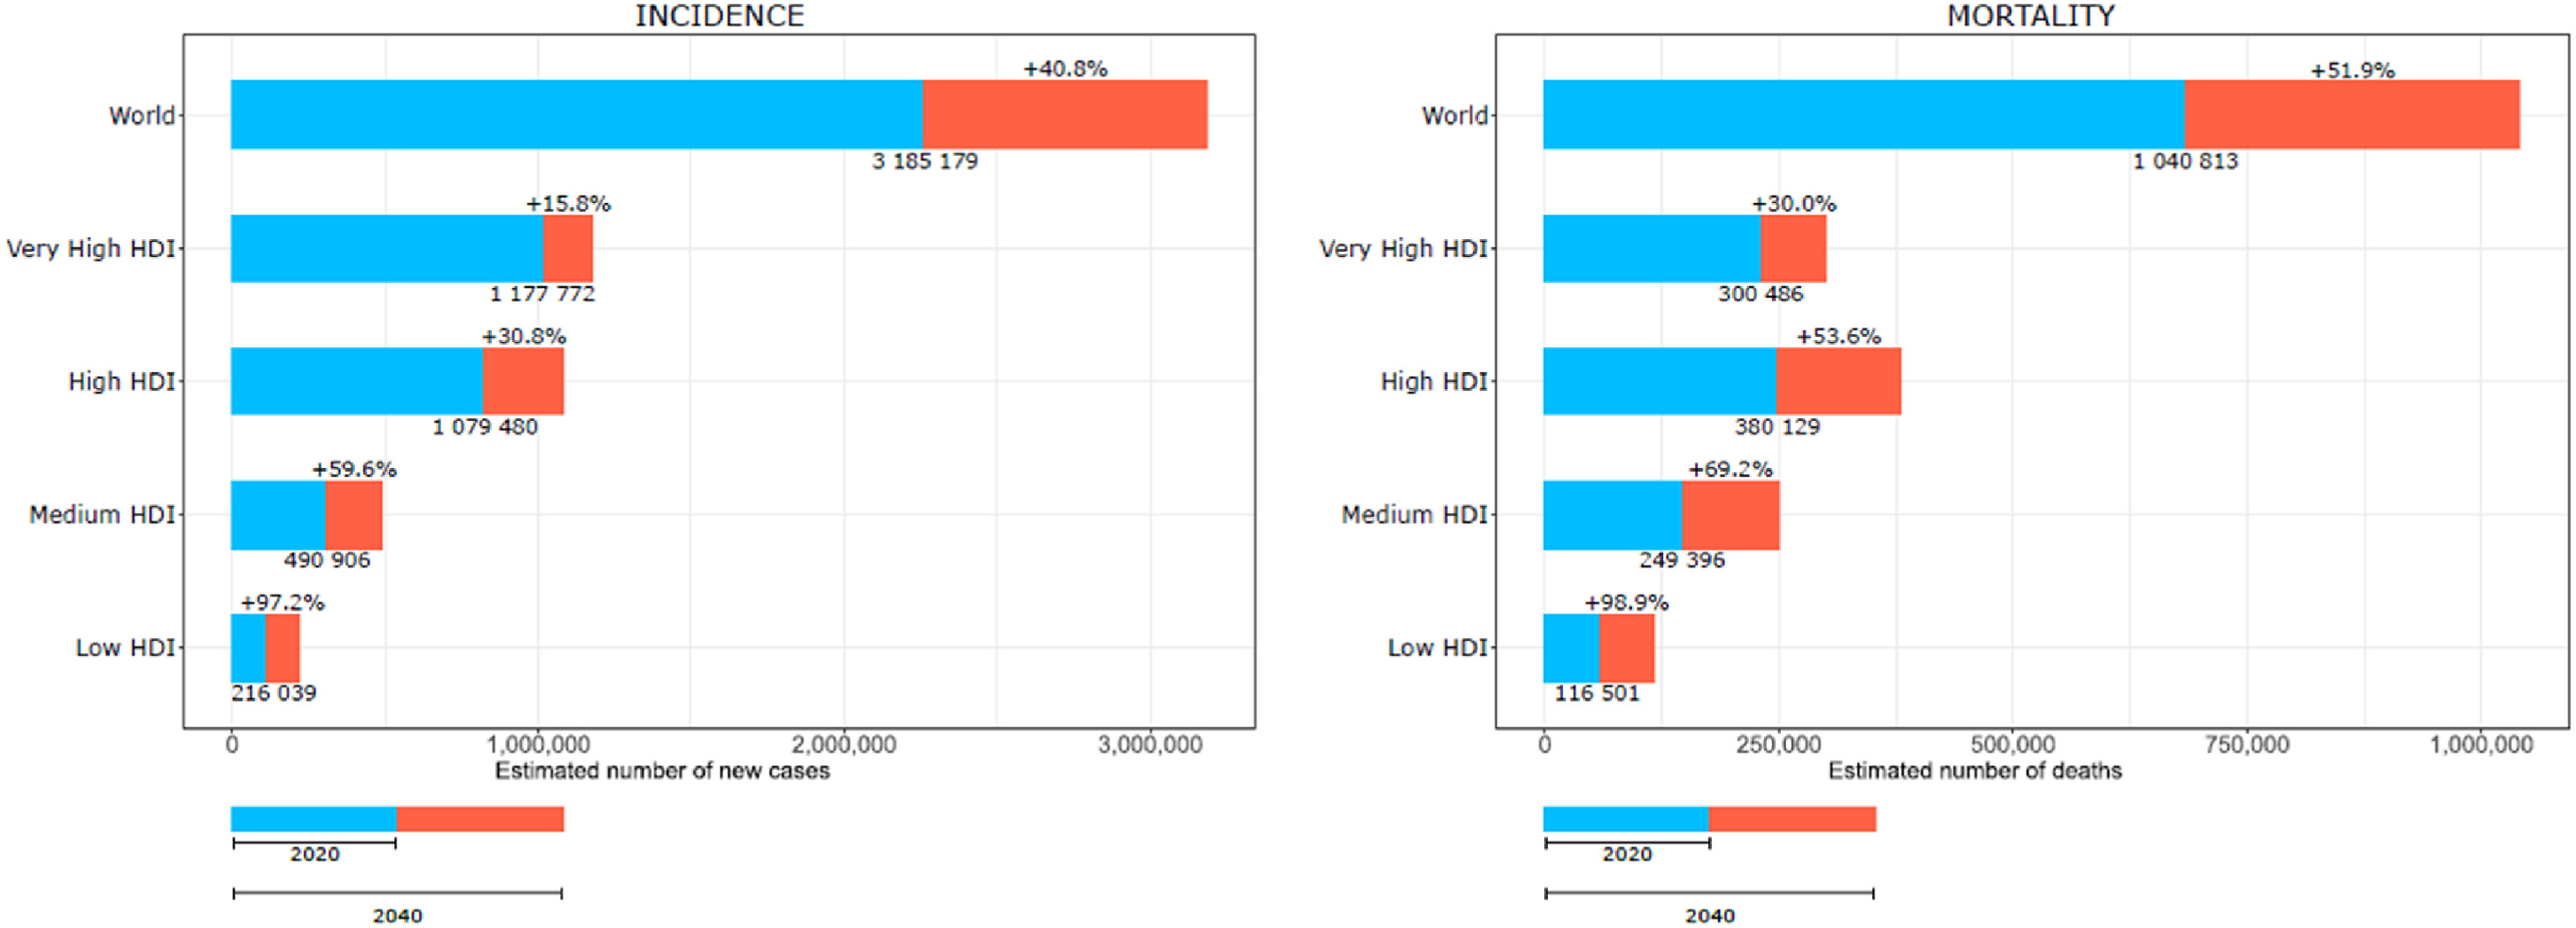
\includegraphics[width=\textwidth]{BC2020-2040.jpg} % Caminho para sua imagem
%     \caption{Projected changes in breast cancer incidence and mortality between 2020 and 2040 across Human Development 
%     Index (HDI) categories. \cite{bca_data_Arnold2022Current}}
%     \label{fig:bc_incidence_mortality}
% \end{figure}

%% Incidencia de cancro -> converter imagem em código LaTeX https://gco.iarc.who.int/media/globocan/factsheets/populations/900-world-fact-sheet.pdf

BC is characterized by marked biological heterogeneity, manifested in multiple molecular subtypes that exhibit distinct 
clinical behaviors \cite{bc_molecular_Perou2000} (Perou \textit{et al.}, 2000). Each subtype exhibits substantial differences in 
terms of tumor aggressiveness, metastatic potential, and behavior to specific therapies 
\cite{bc_subtypes_Prat2015Clinical} (Prat \textit{et al.}, 2015). Thus, accurate classification of these subtypes is essential 
to enable personalized therapeutic approaches, with a direct impact on treatment efficacy and patient prognosis. 
\cite{need_for_subtype_treatments_Testa2020Breast} (Testa \textit{et al.}, 2020).

\subsection{Can we improve the classification of Breast Cancer subtypes?}
Among the emerging candidates for robust biomarkers for the classification of  \gls{BC} subtypes are \gls{miRNAs}, 
small non-coding RNA molecules that play a crucial regulatory role in gene expression. They are estimated to 
modulate the expression of about one-third of the genes in the human genome \cite{mirna_importance_Hammond2015An} 
(Hammond \textit{et al.}, 2015) and are implicated in the regulation of multiple physiological and pathological 
processes, including various human diseases \cite{mirna_as_biomarkers_Ho2022} (Ho \textit{et al.}, 2022).

Given their regulatory nature, several studies have demonstrated a significant association between \gls{miRNAs} expression 
profiles and relevant clinical characteristics in the context of \gls{BC}, including processes such as tumor 
progression and metastasis development \cite{mirna_as_biomarkers_Ho2022} \cite{mirnas_in_bc_Muñoz2023} (Muñoz \textit{et al.}, 2023) \cite{mirna_as_bio_for_sub_Blenkiron2007MicroRNA} (Blenkiron \textit{et al.}, 2007). 
In addition to these aspects, a seminal 
study by Blenkiron \textit{et al.} (2007) demonstrated that \gls{miRNAs} expression profiles can effectively distinguish between 
different molecular subtypes of \gls{BC}, highlighting their potential as a precise subtyping tool. This ability to 
discriminate between subtypes reinforces the value of \gls{miRNAs} as promising clinical biomarkers.

\subsection{How to identify the most relevant miRNAs?}

The identification of the most relevant \gls{miRNAs} for \gls{BC} subtyping represents a major analytical challenge due 
to the complexity of these high dimensional regulatory molecules, non-linearity interactions between and 
clinical phenotypes require advanced computational approaches to be effectively modelled. Recent advances in \gls{AI}, 
particularly in \gls{ML} and \gls{DL}, have demonstrated remarkable potential in extracting meaningful patterns from 
high-dimensional and heterogeneous (data from distinct nature) biomedical data. These approaches enable not only the 
accurate classification of \gls{BC} subtypes but also the identification of discriminative \gls{miRNAs} signatures, 
supporting their integration as actionable biomarkers in clinical workflows.

In this context, \gls{ML} and \gls{DL} models are particularly well suited for the task of robustly characterizing and 
explaining the profiles of \gls{miRNAs}-based biomarkers — should such biomarkers exist — with the potential to effectively 
discriminate between different \gls{BC} subtypes, as already seen in a study done by  \cite{ml_gastric_Azari2023} Azari \textit{et al.} 2023 where \gls{ML} 
algorithms identified potential diagnostic and prognostic \glossary{miRNAs} in gastric cancer, showing high accuracy in the 
identification of reliable biomarkers for this disease.

This reality reinforces the urgency of developing advanced computational tools that can enable more precise molecular 
characterization and guide personalized therapeutic decisions, ultimately improving clinical outcomes for patients with 
aggressive and hard-to-treat \gls{BC} subtypes.
